\usetikzlibrary{arrows.meta,calc}
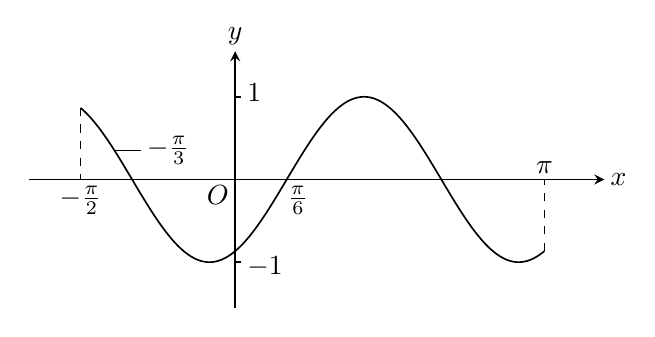
\begin{tikzpicture}[x=1.25cm,y=1.05cm,line width=.6pt,>=stealth]
\draw[->] (-2.1,0)--(3.75,0) node[right,inner sep=0pt,xshift=2pt] {$x$};
\draw[->] (0,-1.55)--(0,1.55) node[above,inner sep=0pt,yshift=2pt] {$y$};
\draw (0,1)--(0.06,1);
\draw (0,-1)--(0.06,-1);
\node[right,inner sep=0pt,xshift=2pt,yshift=1.5pt] at (0.06,1) {$1$};
\node[right,inner sep=0pt,xshift=2pt,yshift=-1.5pt] at (0.06,-1) {$-1$};
\node[below left,inner sep=0pt,xshift=-2pt,yshift=-2pt] at (0,0) {$O$};
\draw[domain=-1.5707963:3.1415927,samples=220] plot (\x,{sin(deg(2*\x-pi/3))});
\draw[dashed,line width=.45pt] (-1.5707963,0.8660254)--(-1.5707963,0);
\draw[dashed,line width=.45pt] (3.1415927,-0.8660254)--(3.1415927,0);
\node[below,inner sep=0pt,yshift=-2pt] at (-1.5707963,0) {$-\frac{\pi}{2}$};
\draw[line width=.45pt] (-1.2261,0.35)--(-0.96,0.35);
\node[anchor=west,inner sep=0pt,xshift=2pt] at (-0.96,0.35) {$-\frac{\pi}{3}$};
\node[below,inner sep=0pt,xshift=4pt,yshift=-2pt] at (0.5235988,0) {$\frac{\pi}{6}$};
\node[above,inner sep=0pt,yshift=2pt] at (3.1415927,0) {$\pi$};
\end{tikzpicture}
